
\section{Procedure for Linux}

\begin{itemize}
	
\item Go to \url{https://kat-cpt-vpn.kat.ac.za}
\item Log in using your credentials provided to you.
\item Go to the''\sensor{Configurations}' link.
\item Click on 'Continue...', type a name in the 'Name' field and then click ‘Create and Download’. This will create a .ovpn config file with the name as provided in the 'Name' field and prompt you to download the file.
\item When prompted, save the file somewhere on your drive (the 'Home' directory is a good place as the terminal usually opens up with the Home directory as the default directory)
\item Assuming you have OpenVPN installed, open a terminal session and type:
\begin{lstlisting}[style=DOS]
sudo openvpn --config 'filePath/fileName.ovpn'
\end{lstlisting}

	where 'filePath' is the directory in which the config file is saved and 'fileName' is the       name of the config file downloaded. For example if the name of the config file is 'SiteVPN' and it was saved in the home directory of a computer whose user is called 'admin', then the command will be as follows:
\begin{lstlisting}[style=DOS]
sudo openvpn --config 'home/admin/SiteVPN.ovpn'
\end{lstlisting}

Once command is executed and the last line is:
\begin{lstlisting}[style=DOS]
Initialization Sequence Completed
\end{lstlisting}

	then you are connected.
\item If you do not have Openvpn installed, then follow the steps below:
\begin{itemize}
\item[$\circ$] After downloading the .ovpn config file, go to VPN settings

\begin{figure}[!thb]
	\centering
	%\includegraphicsdpi{100}{}{bur1.png}     
	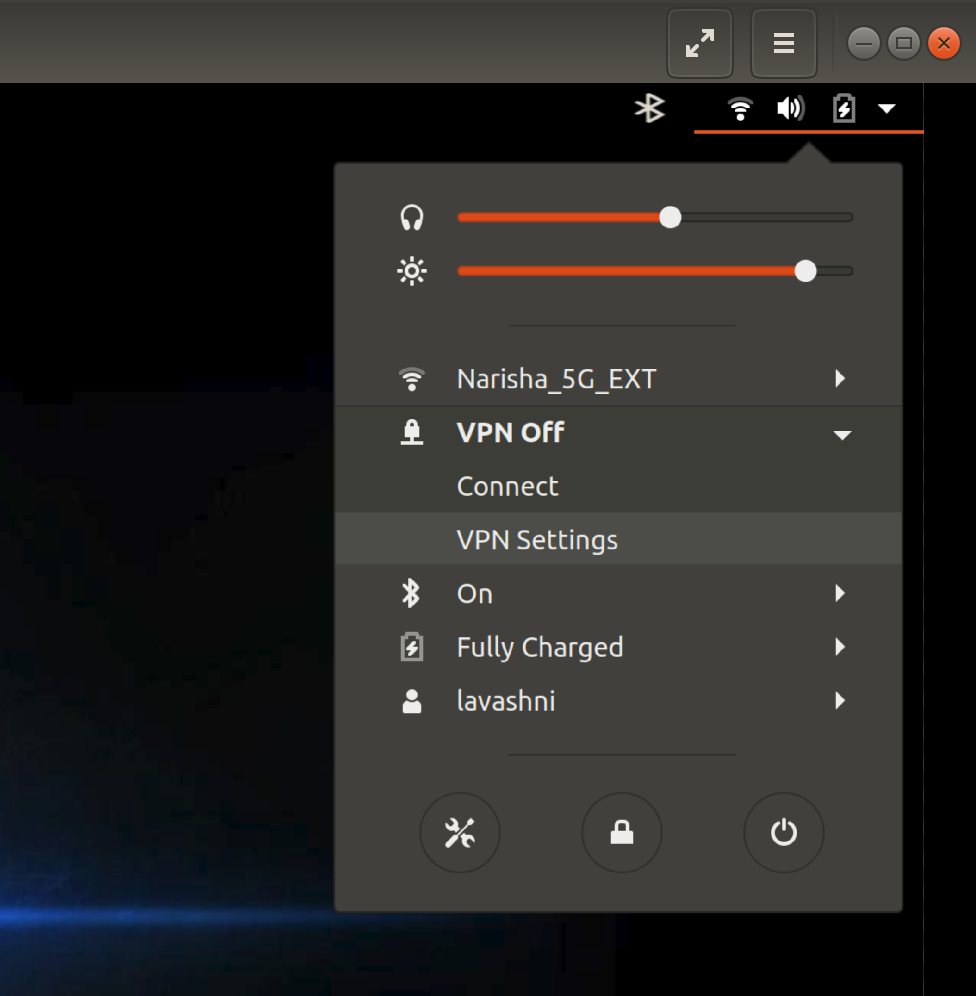
\includegraphics[scale=0.25]{Chapters/images/image39.png}
	
	%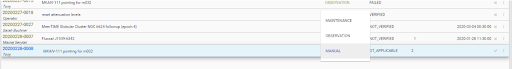
\includegraphics[resolution=100]{bur1.png}
	\caption{Linux VPN settings }
	\label{fig:image39}
\end{figure}


\item[$\circ$] Click on the ‘plus’ sign to add VPN

\begin{figure}[!thb]
	\centering
	%\includegraphicsdpi{100}{}{bur1.png}     
	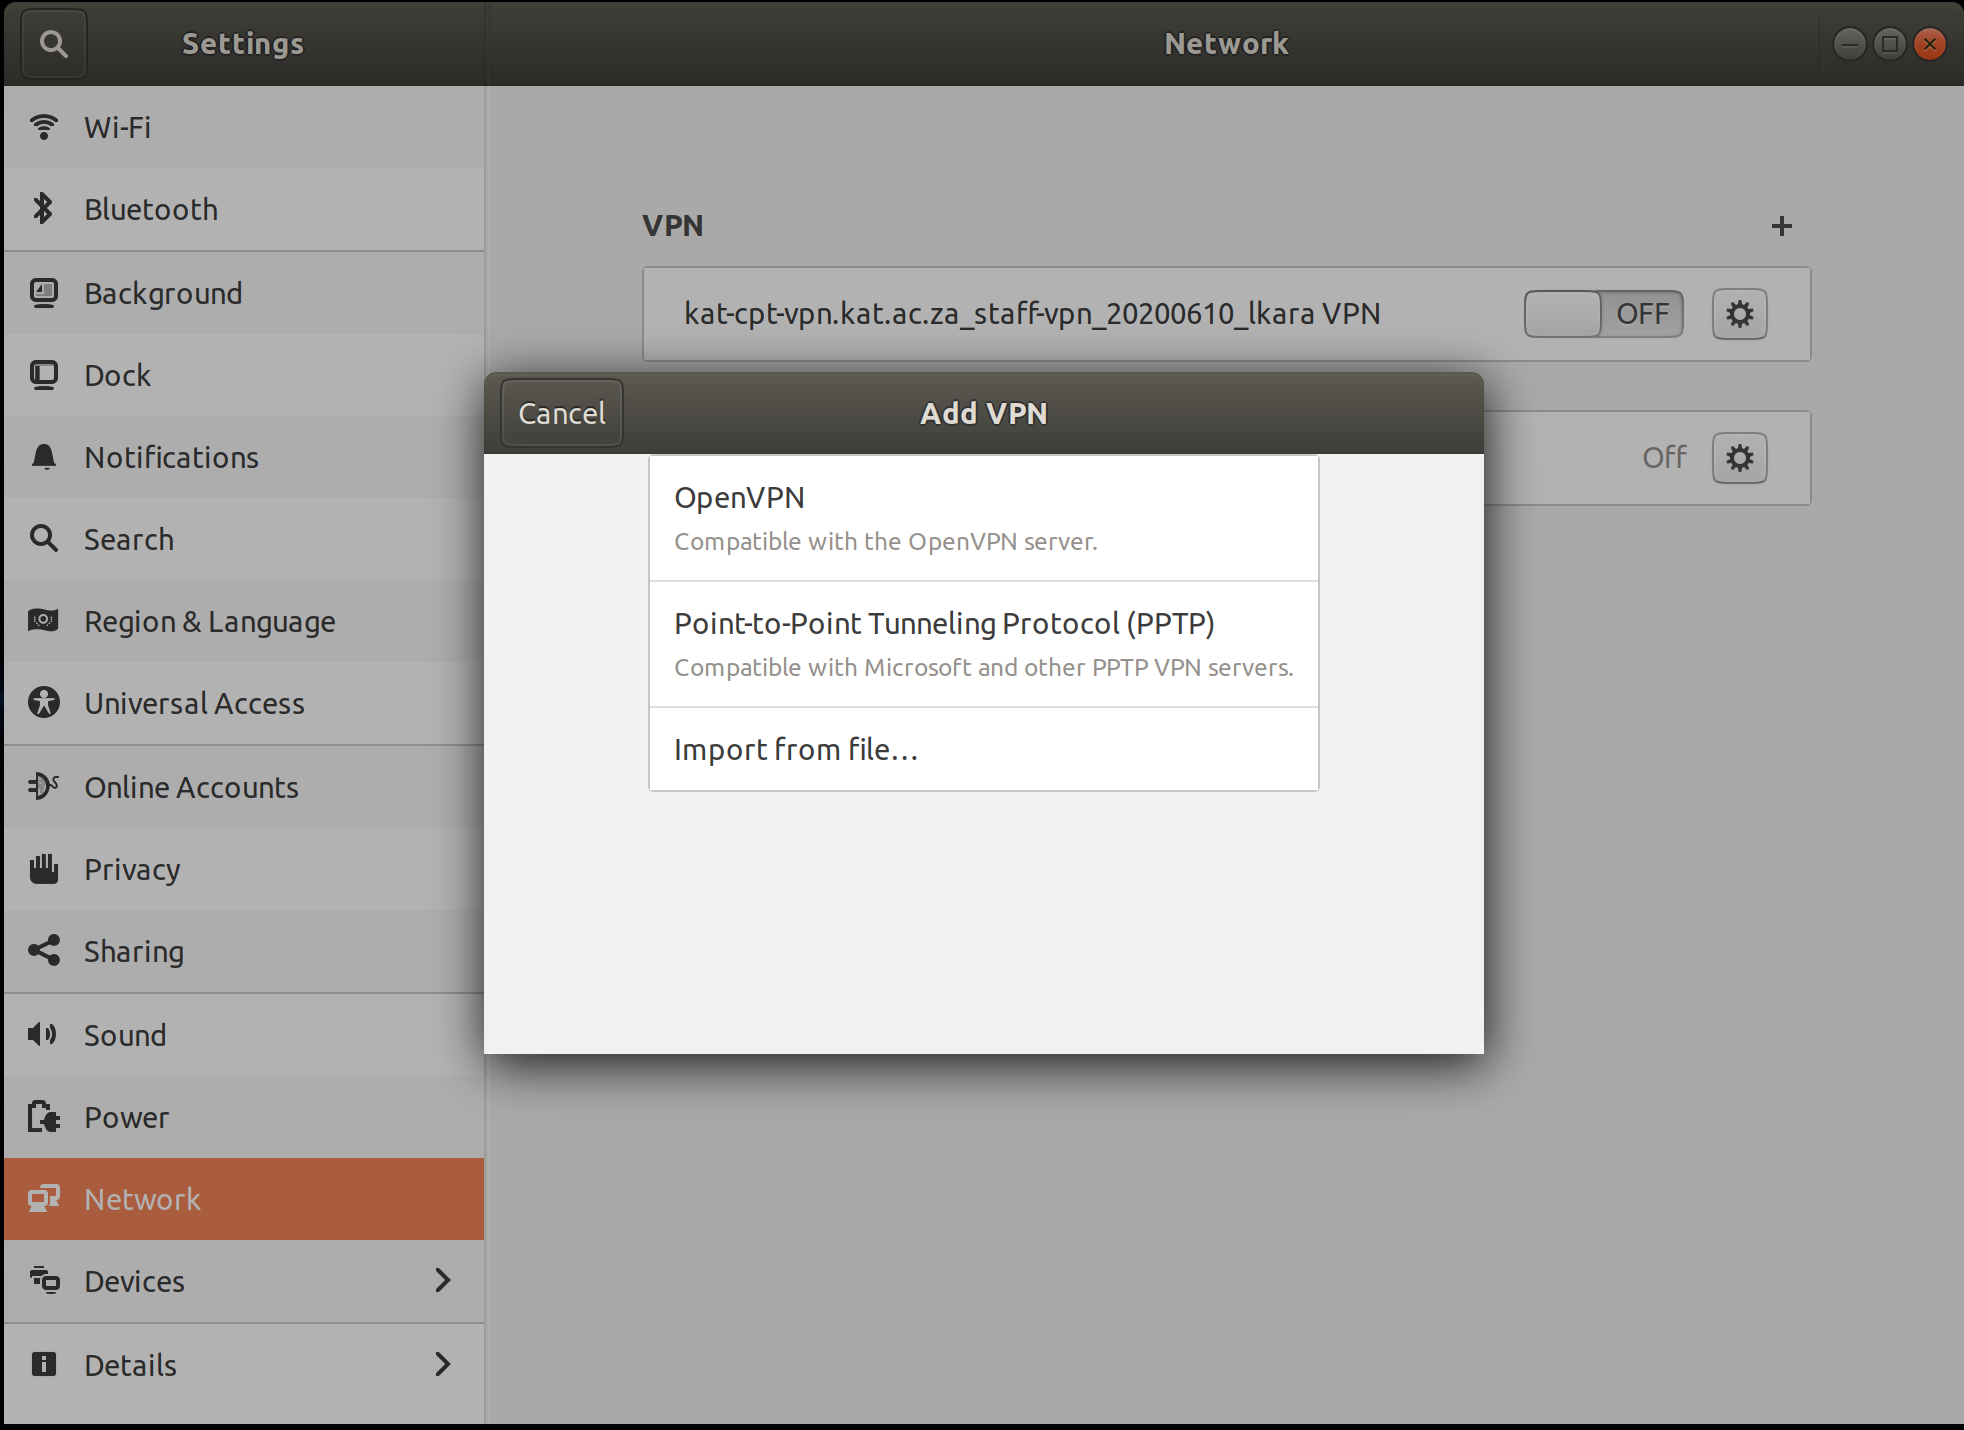
\includegraphics[scale=0.25]{Chapters/images/image2.png}
	
	%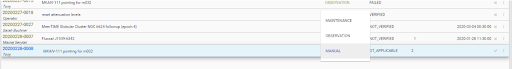
\includegraphics[resolution=100]{bur1.png}
	\caption{Linus add vpn dialog box}
	\label{fig:image2}
\end{figure}

\item[$\circ$] Select ‘Import from file...’, you will be directed to your ‘Home’ folders so that you can choose the correct file to import
\begin{figure}[!thb]
	\centering
	%\includegraphicsdpi{100}{}{bur1.png}     
	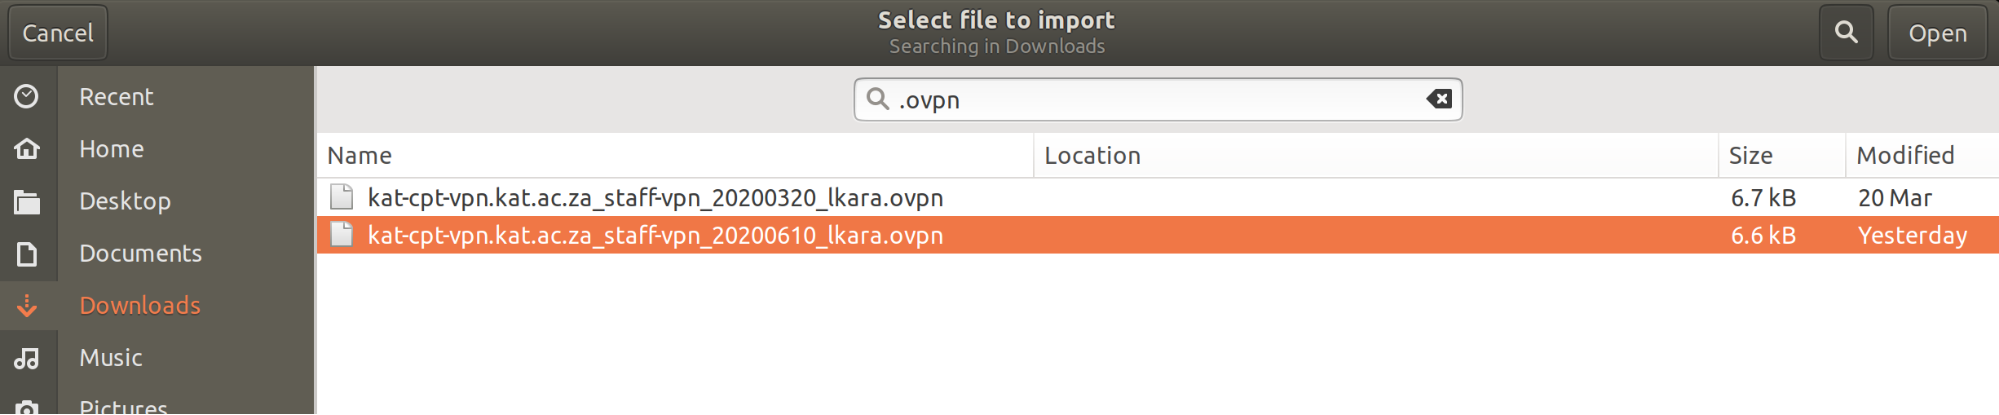
\includegraphics[scale=0.23]{Chapters/images/image130.png}
	
	%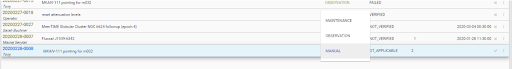
\includegraphics[resolution=100]{bur1.png}
	\caption{CAM GUI approved SB }
	\label{fig:image130}
\end{figure}


\item[$\circ$] After clicking on the correct .ovpn config file, the following window should appear

\begin{figure}[!thb]
	\centering
	%\includegraphicsdpi{100}{}{bur1.png}     
	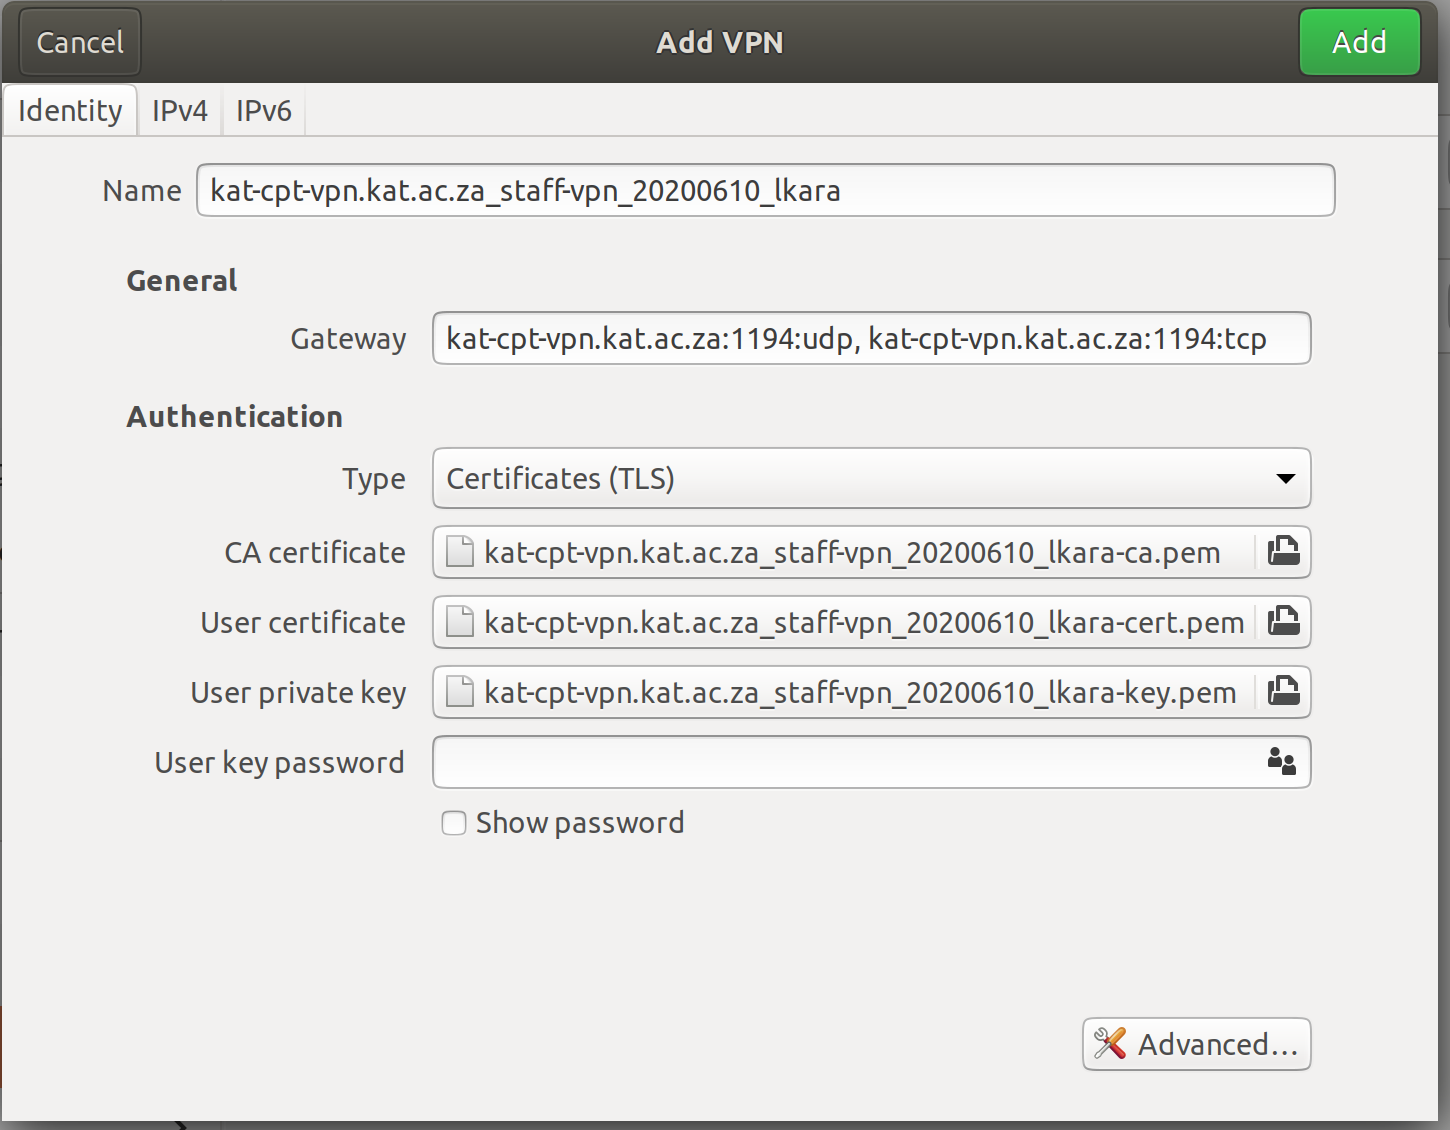
\includegraphics[scale=0.25]{Chapters/images/image112.png}
	
	%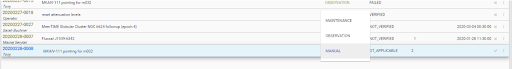
\includegraphics[resolution=100]{bur1.png}
	\caption{CAM GUI approved SB }
	\label{fig:image112}
\end{figure}

\item[$\circ$] All of the information from the .ovpn config file has  automatically been filled in, all you need to do is click ‘Add’.

\item[$\circ$] You will see the name of the latest .ovpn config file installed (don't forget to remove the old .ovpn config file).
\begin{figure}[!thb]
	\centering
	%\includegraphicsdpi{100}{}{bur1.png}     
	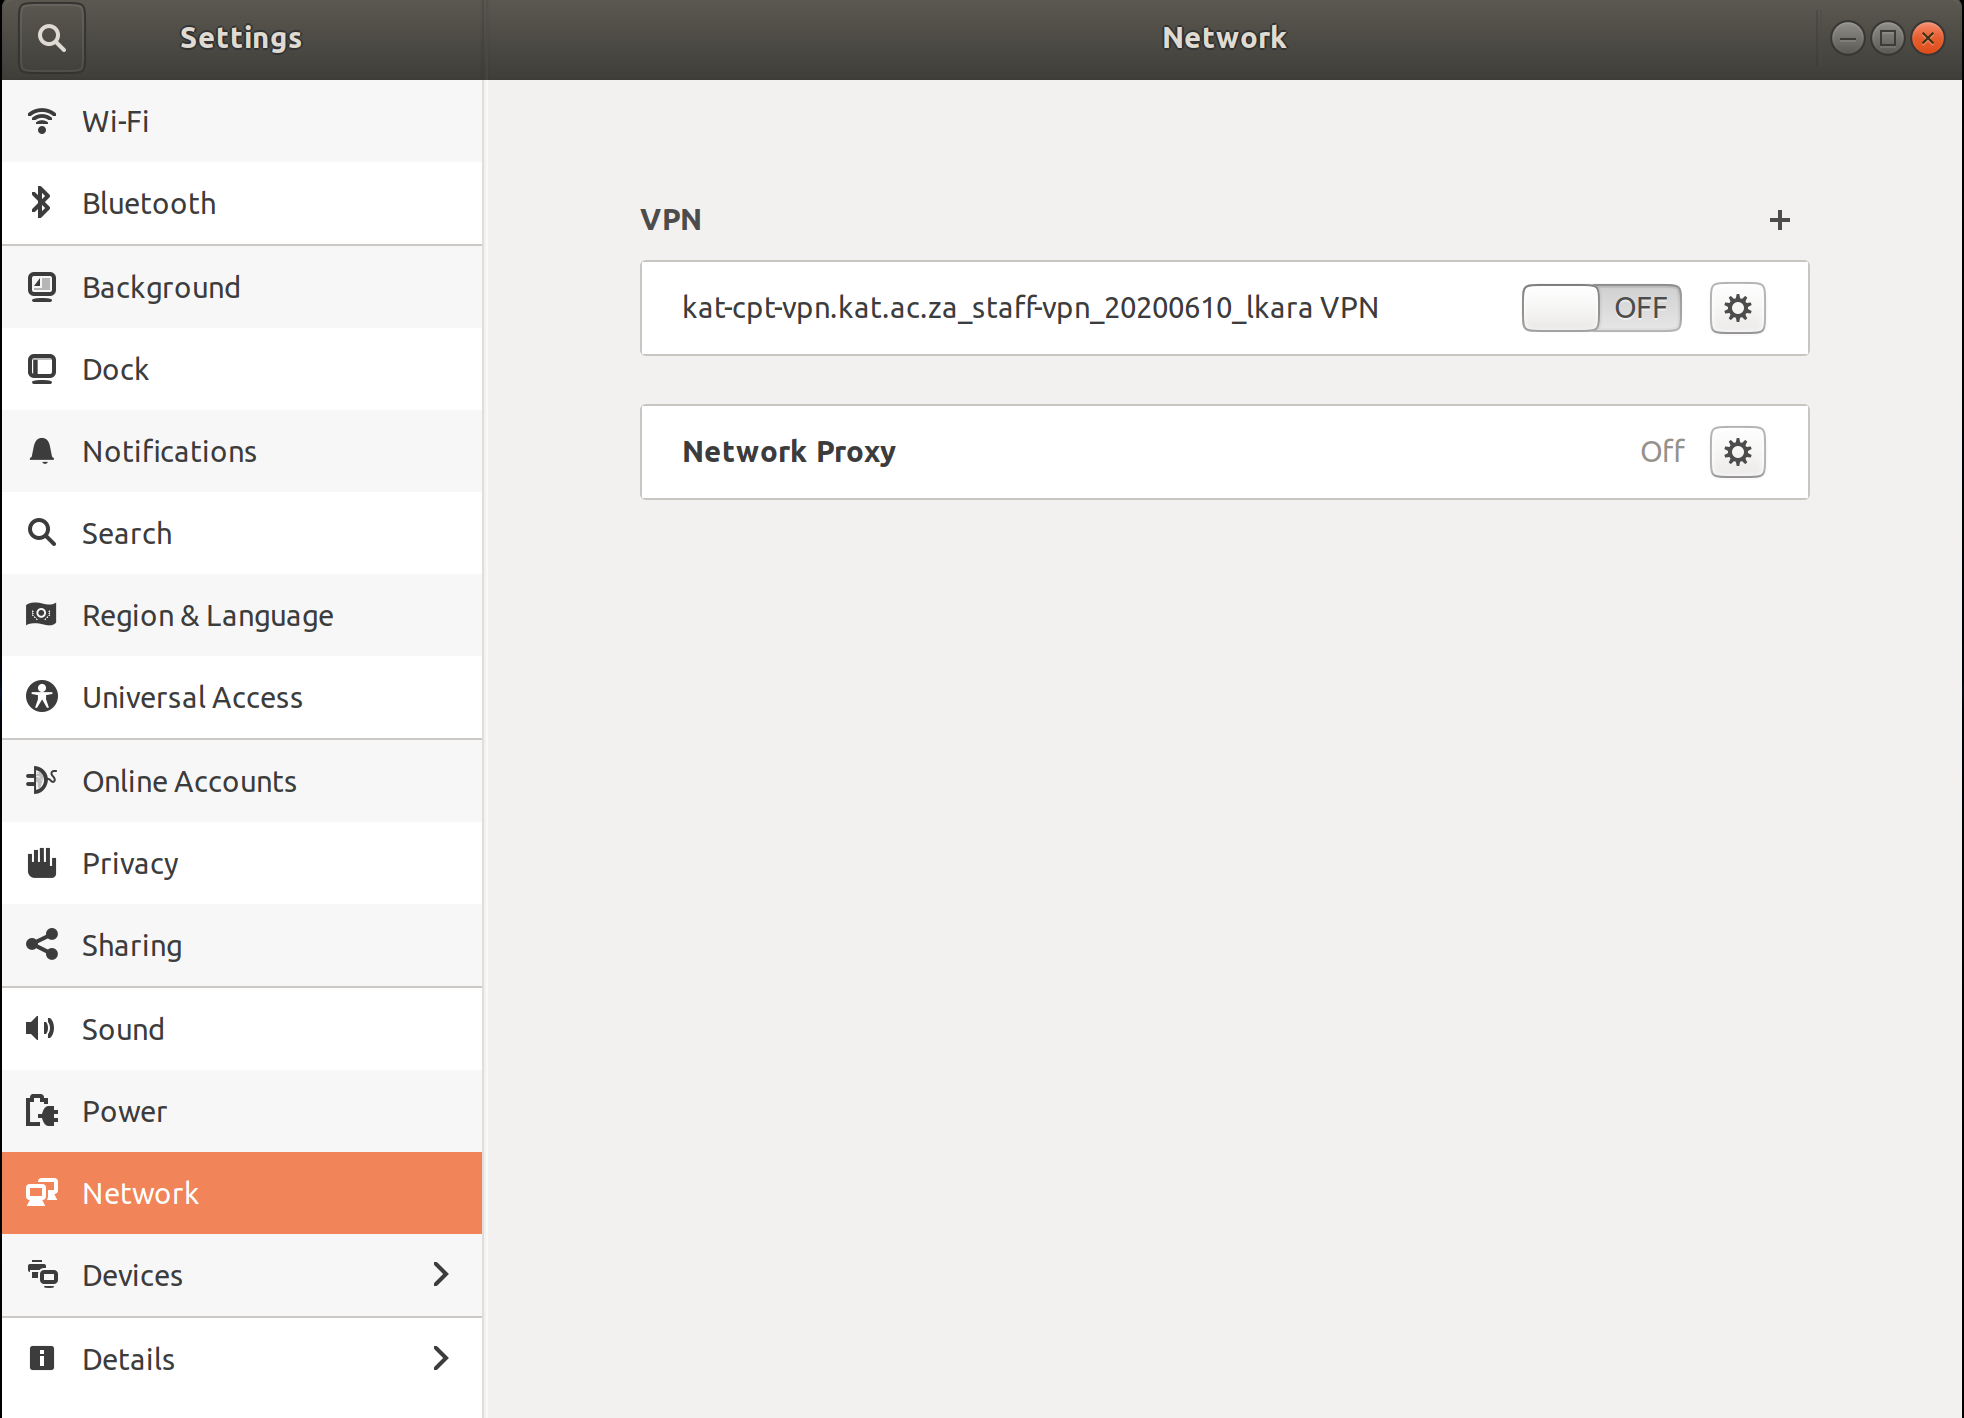
\includegraphics[scale=0.25]{Chapters/images/image60.png}
	
	%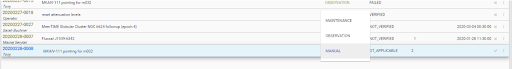
\includegraphics[resolution=100]{bur1.png}
	\caption{CAM GUI approved SB }
	\label{fig:image60}
\end{figure}


\item[$\circ$] You can now connect to VPN 
\end{itemize}
\begin{figure}[!thb]
	\centering
	%\includegraphicsdpi{100}{}{bur1.png}     
	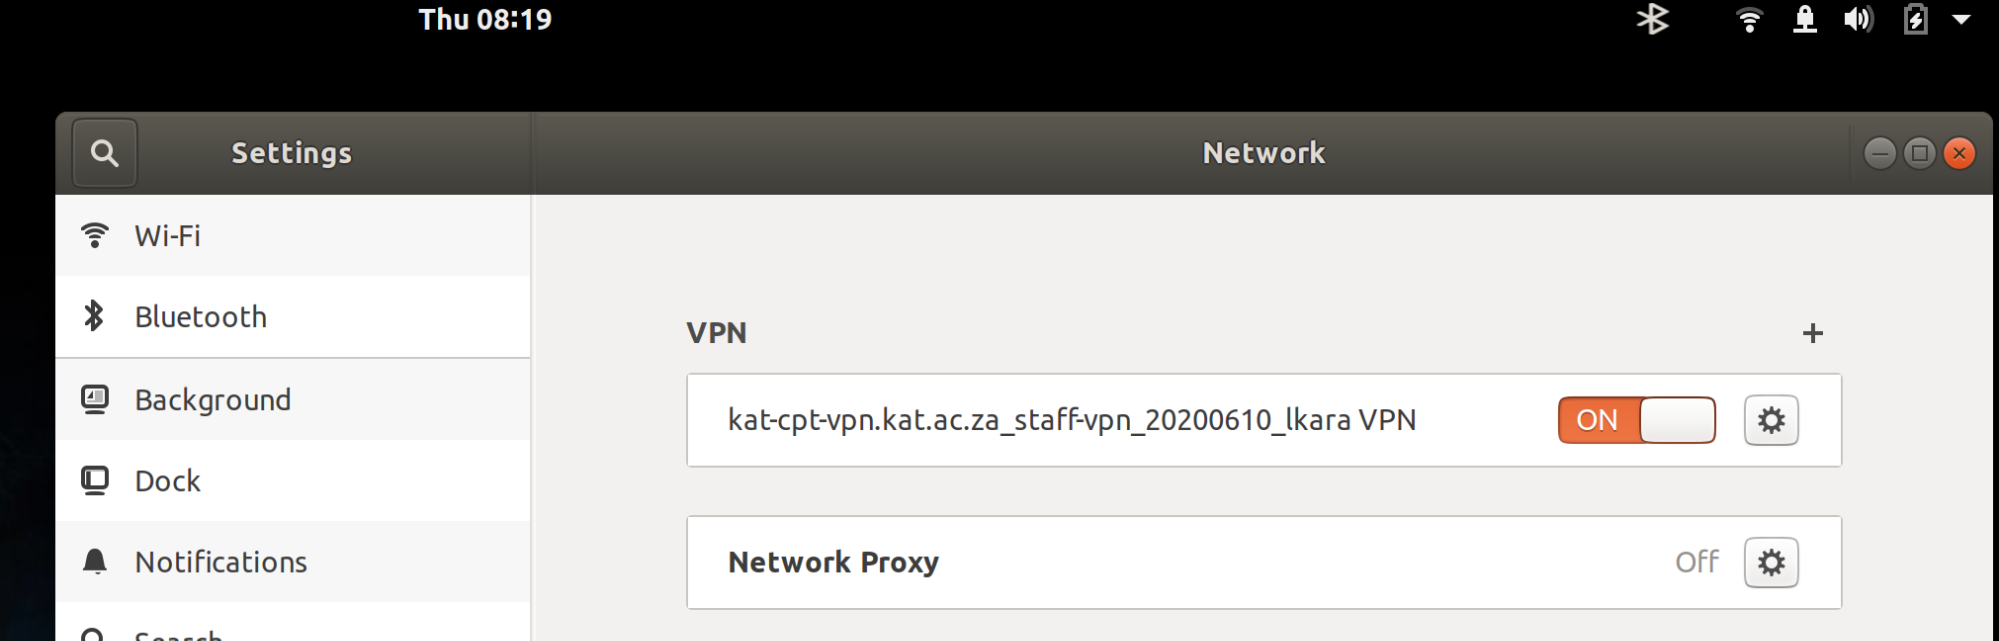
\includegraphics[scale=0.25]{Chapters/images/image101.png}
	
	%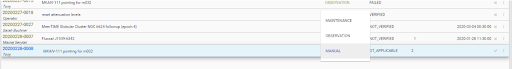
\includegraphics[resolution=100]{bur1.png}
	\caption{CAM GUI approved SB }
	\label{fig:image101}
\end{figure}

\item Don’t forget to delete the old configuration every time that you download a new one on the EduVPN site
\begin{figure}[!thb]
	\centering
	%\includegraphicsdpi{100}{}{bur1.png}     
	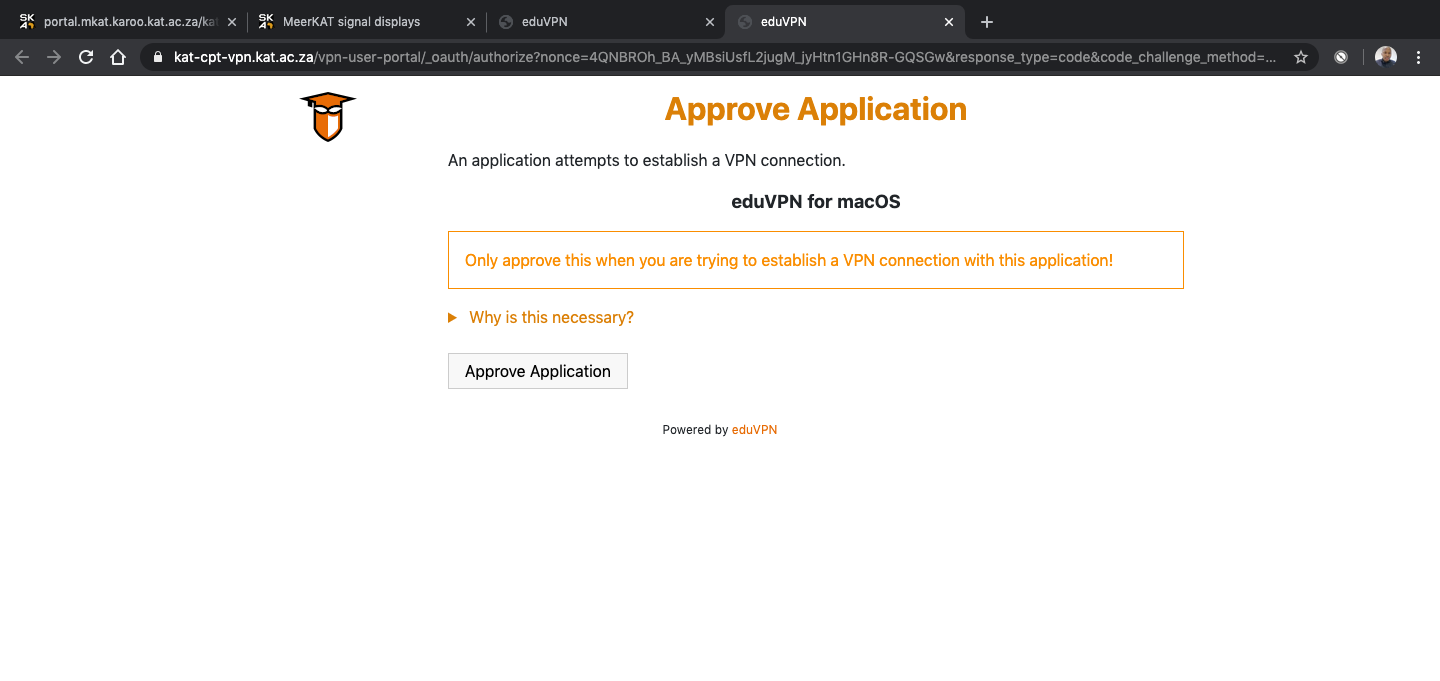
\includegraphics[scale=0.25]{Chapters/images/image26.png}
	
	%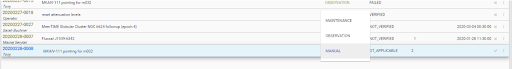
\includegraphics[resolution=100]{bur1.png}
	\caption{Linux EduVPN approve dialog box }
	\label{fig:image26}
\end{figure}

\end{itemize}


\section{Procedure for MacOS}
Download the EduVPN macOS Software from\\ \url{https://kat-cpt-vpn.kat.ac.za/vpn-user-portal/home}

\begin{figure}[!thb]
	\centering
	%\includegraphicsdpi{100}{}{bur1.png}     
	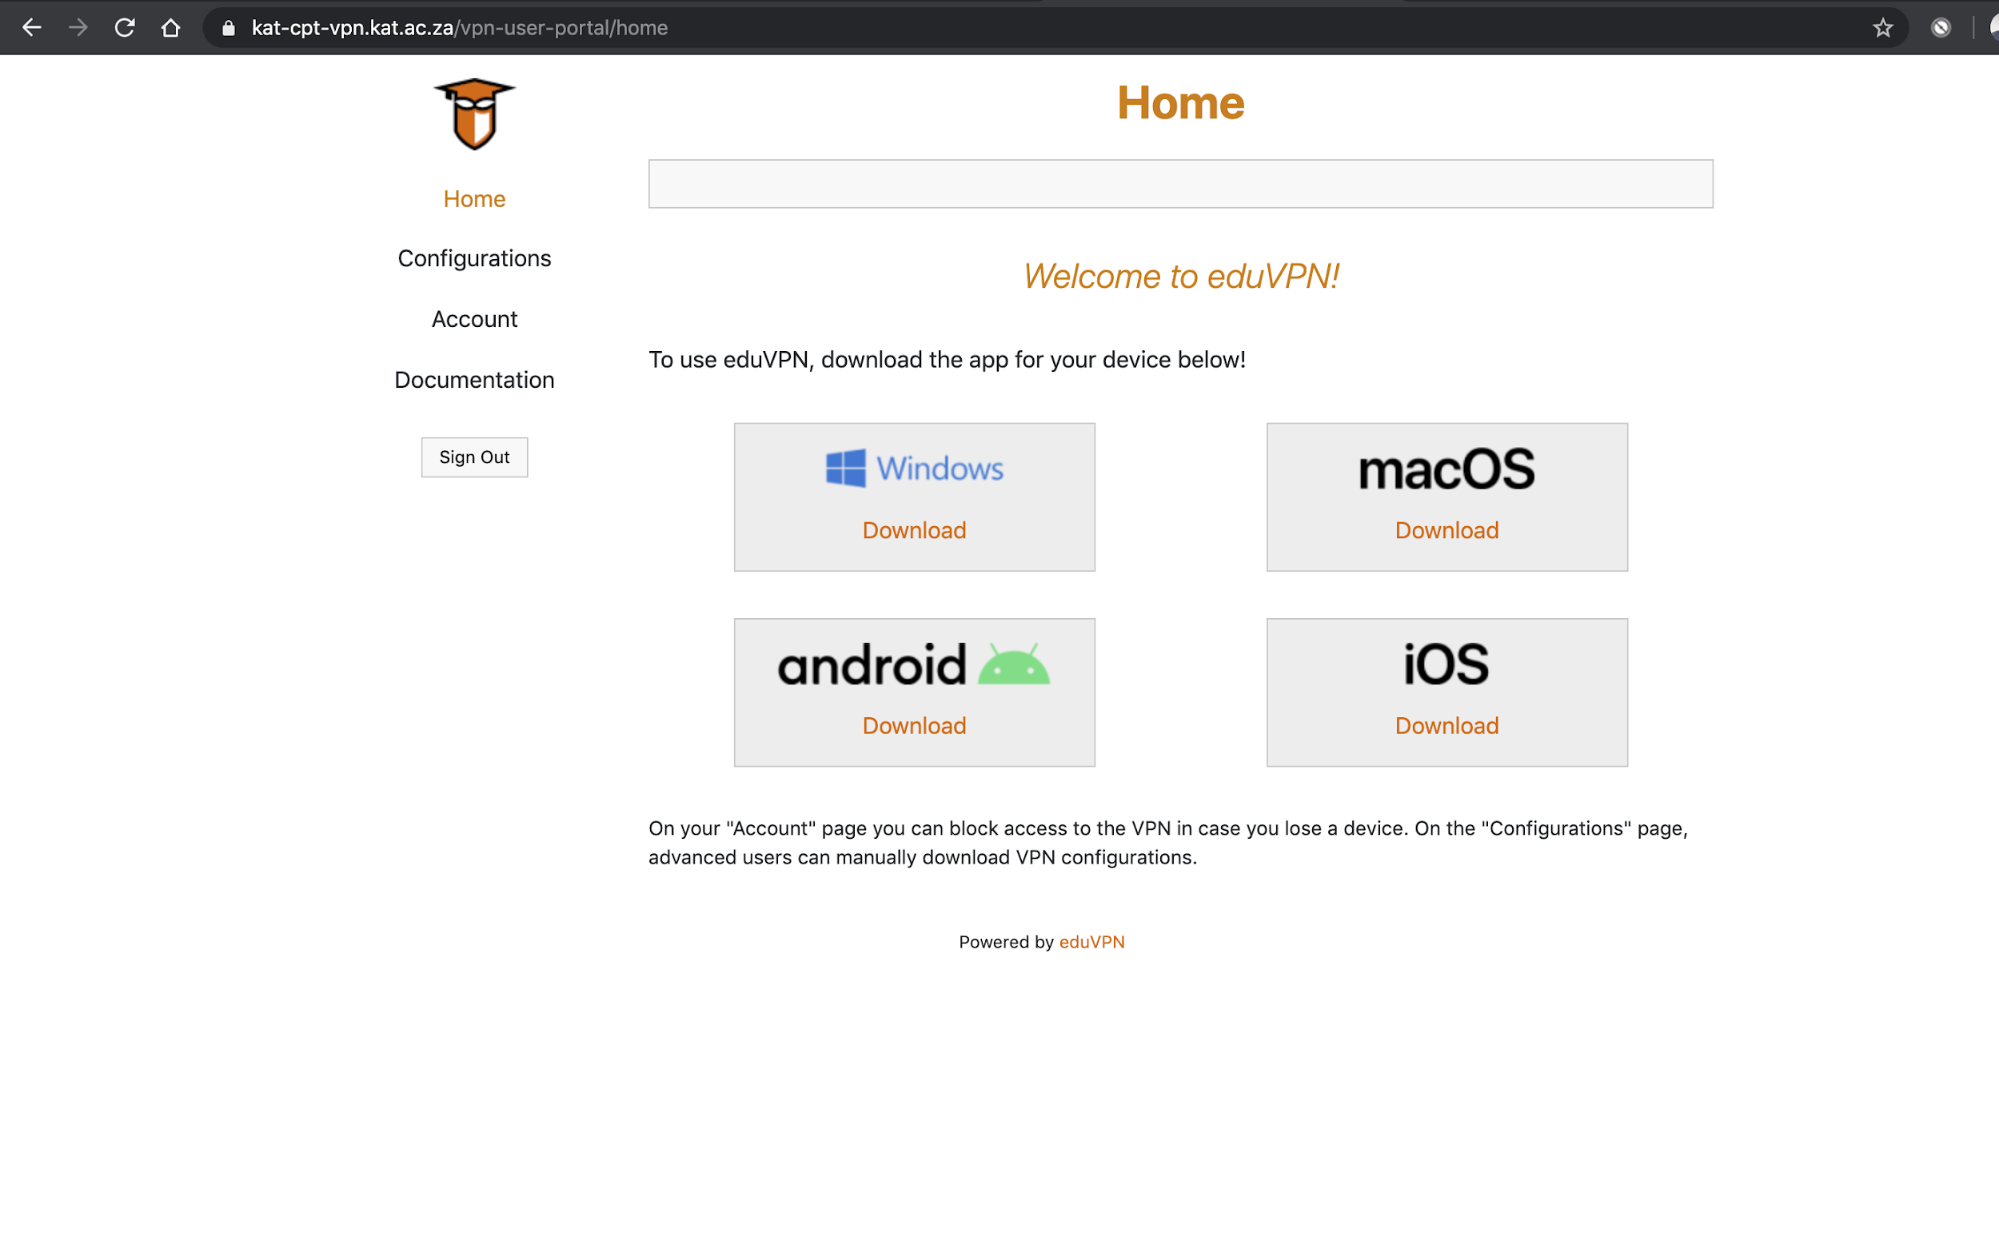
\includegraphics[scale=0.23]{Chapters/images/image106.png}
	
	%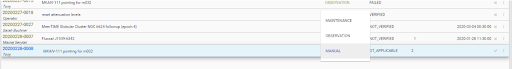
\includegraphics[resolution=100]{bur1.png}
	\caption{MacOS EduVPN download page }
	\label{fig:image106}
\end{figure}


Install and run the software.



\begin{figure}[!thb]
	\centering
	%\includegraphicsdpi{100}{}{bur1.png}     
	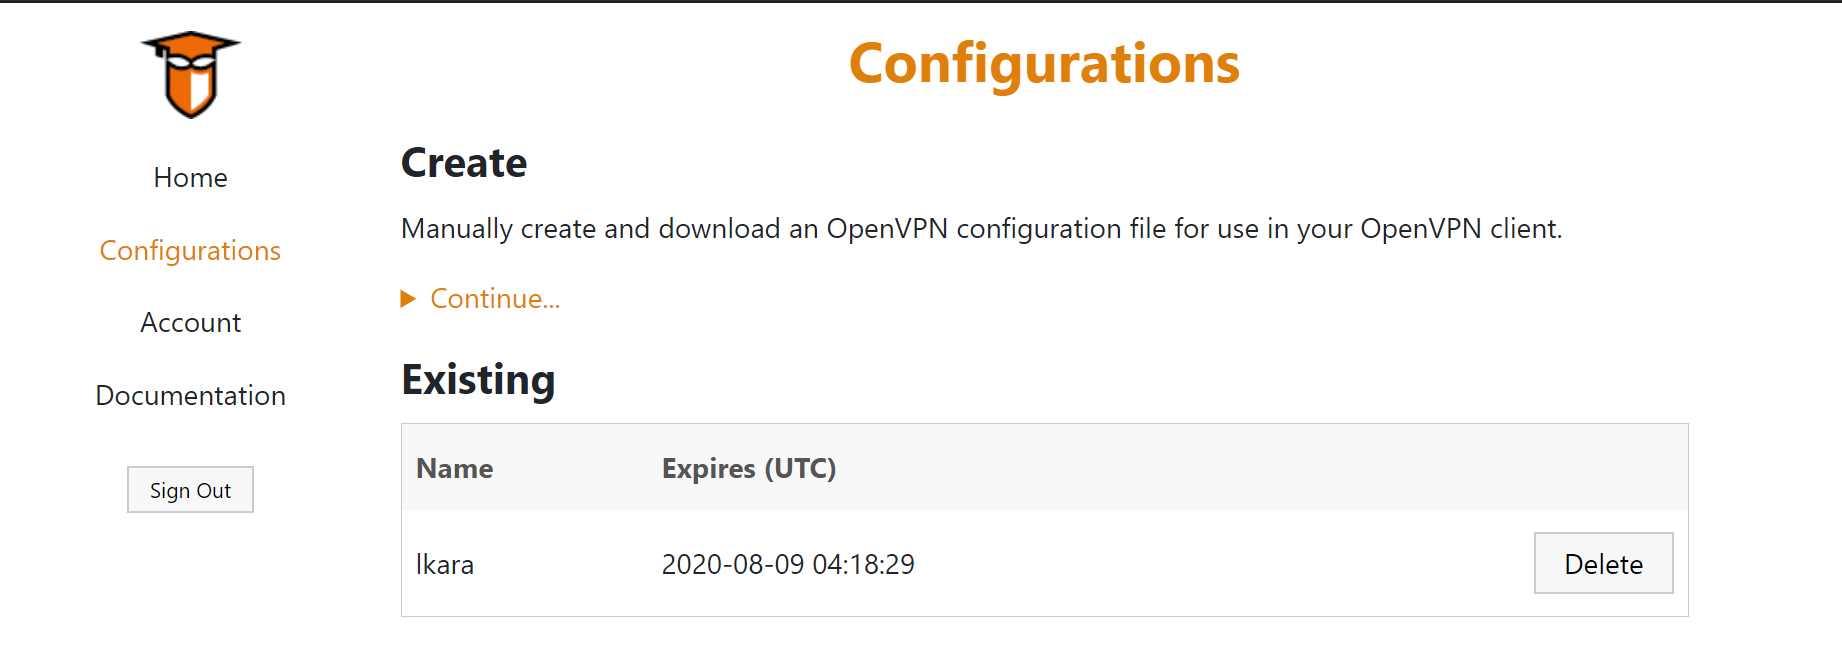
\includegraphics[scale=0.23]{Chapters/images/image45.png}
	
	%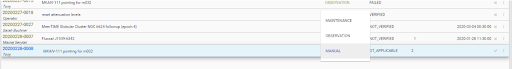
\includegraphics[resolution=100]{bur1.png}
	\caption{CAM GUI approved SB }
	\label{fig:image45}
\end{figure}

\begin{figure}[!thb]
	\centering
	%\includegraphicsdpi{100}{}{bur1.png}     
	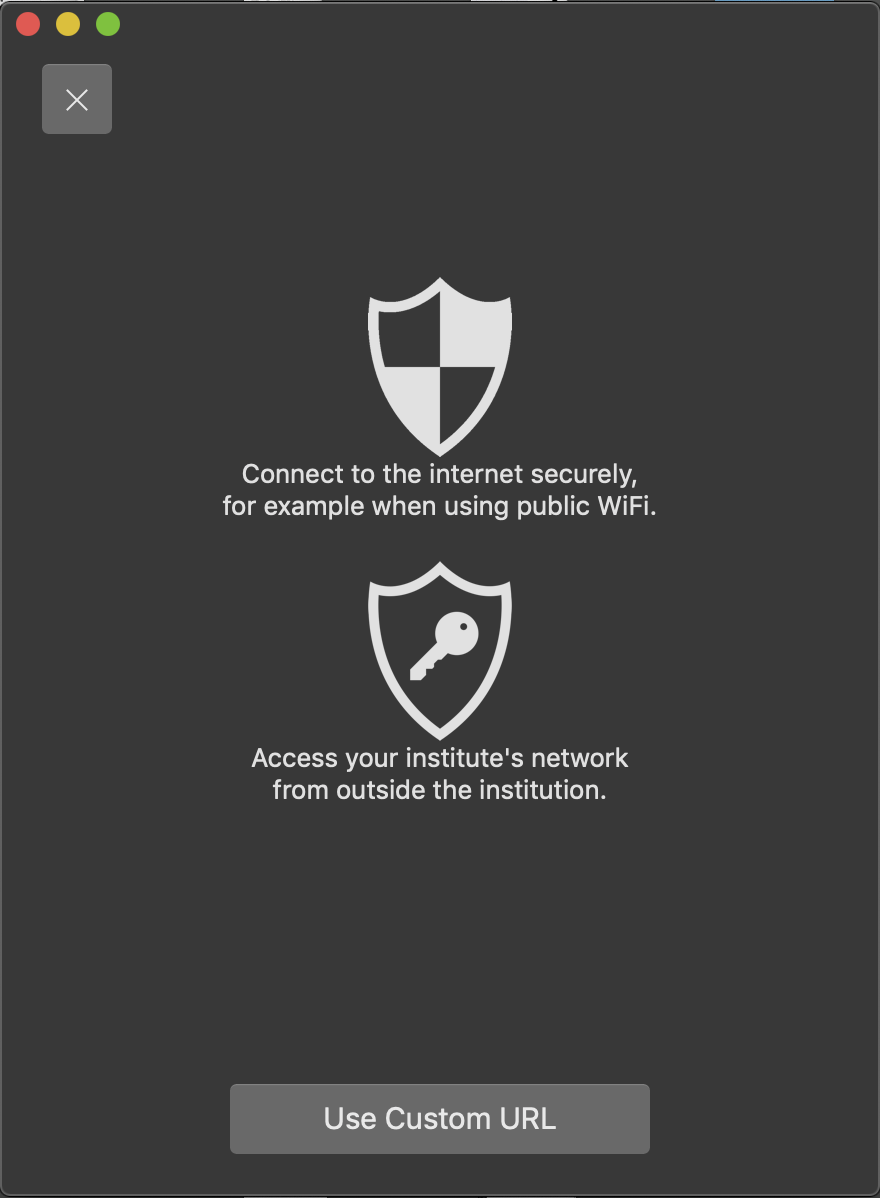
\includegraphics[scale=0.23]{Chapters/images/image105.png}
	
	%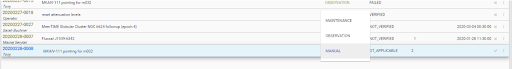
\includegraphics[resolution=100]{bur1.png}
	\caption{MacOS EduVPN download page }
	\label{fig:image105}
\end{figure}

Click "Use Custom URL"\\
Add  \url{https://kat-cpt-vpn.kat.ac.za} to the "Enter URL"


\begin{figure}[!thb]
	\centering
	%\includegraphicsdpi{100}{}{bur1.png}     
	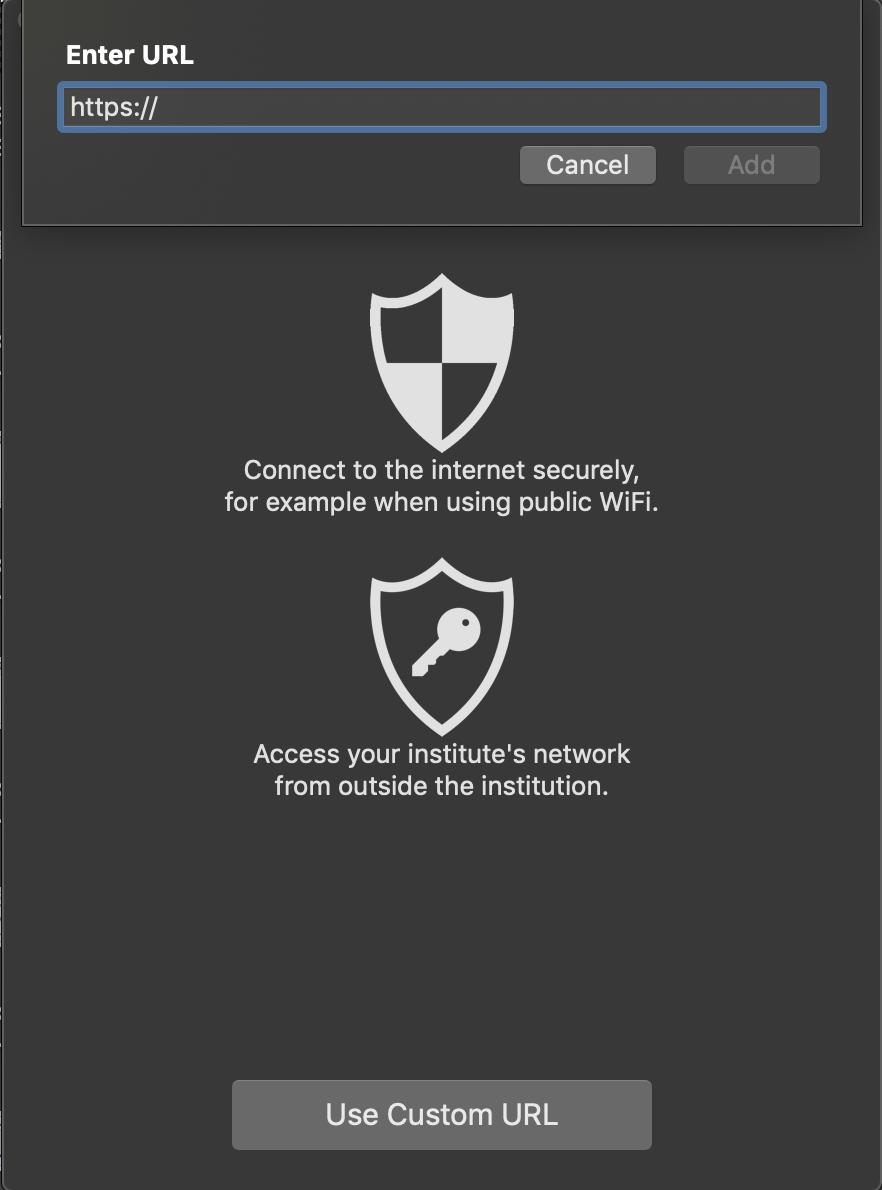
\includegraphics[scale=0.8]{Chapters/images/image74.png}
	
	%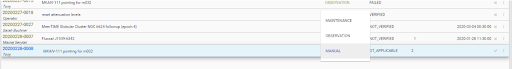
\includegraphics[resolution=100]{bur1.png}
	\caption{CAM GUI approved SB }
	\label{fig:image74}
\end{figure}








\begin{figure}[!thb]
	\centering
	%\includegraphicsdpi{100}{}{bur1.png}     
	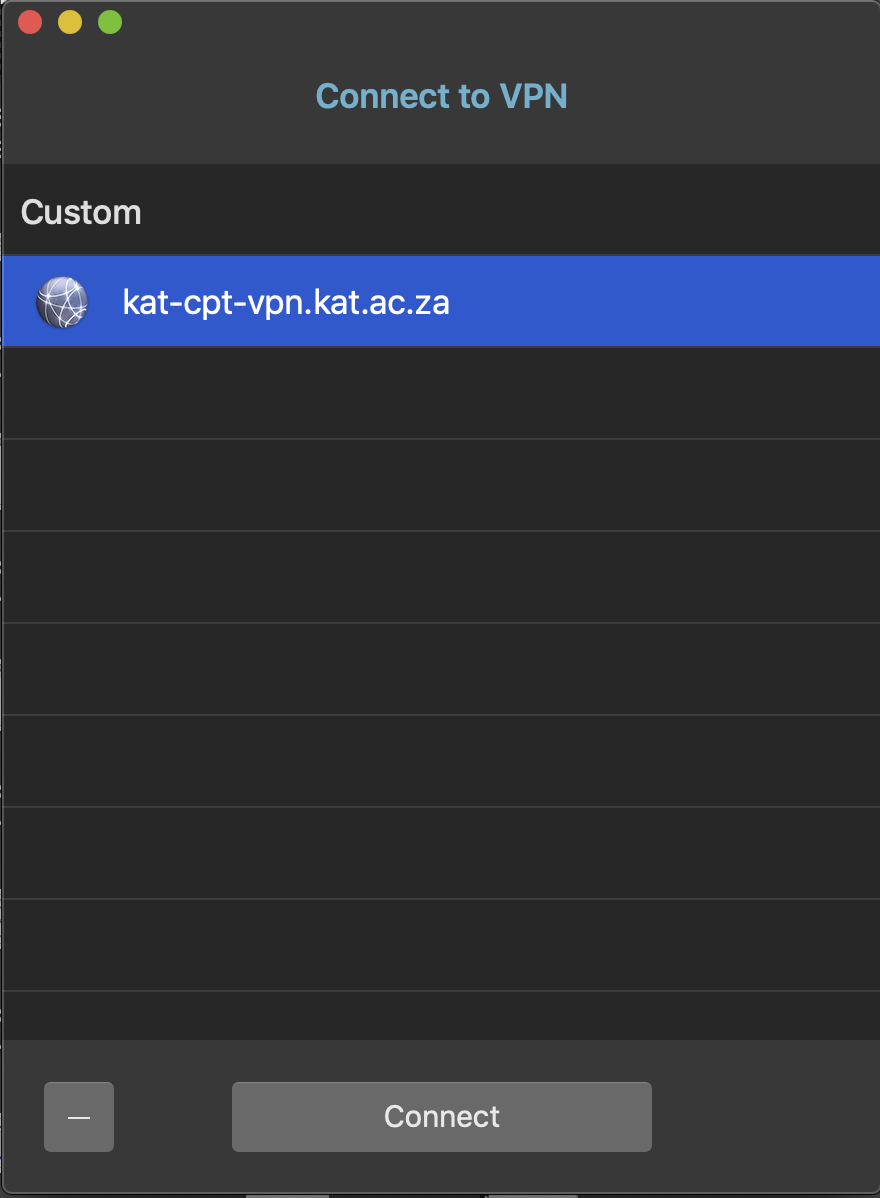
\includegraphics[scale=0.5]{Chapters/images/image63.png}
	
	%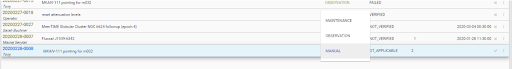
\includegraphics[resolution=100]{bur1.png}
	\caption{CAM GUI approved SB }
	\label{fig:image63}
\end{figure}

Press connect
Once connected to VPN go to https://ipa.kat.ac.za/ipa/ui to set a permanent and secure password for yourself that you will remember.
If you already have an account but eduVPN couldn't connect
Go to https://kat-cpt-vpn.kat.ac.za/vpn-user-portal/account and press Revoke


\begin{figure}[!thb]
	\centering
	%\includegraphicsdpi{100}{}{bur1.png}     
	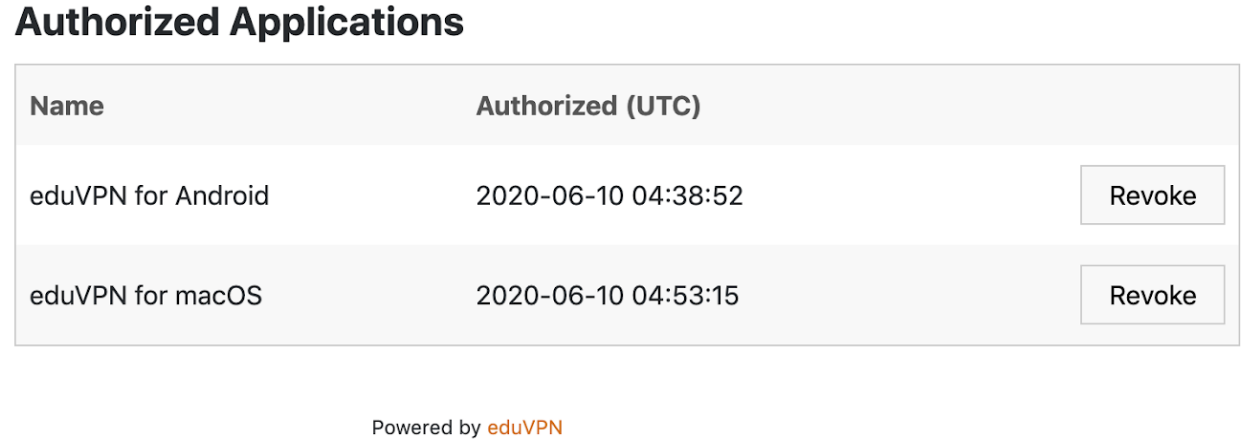
\includegraphics[scale=0.3]{Chapters/images/revoke2.png}
	
	%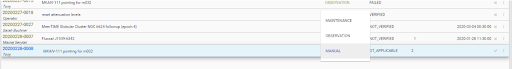
\includegraphics[resolution=100]{bur1.png}
	\caption{CAM GUI approved SB }
	\label{fig:revoke}
\end{figure}






After pressing connect. This message will be displayed
\begin{figure}[!thb]
	\centering
	%\includegraphicsdpi{100}{}{bur1.png}     
	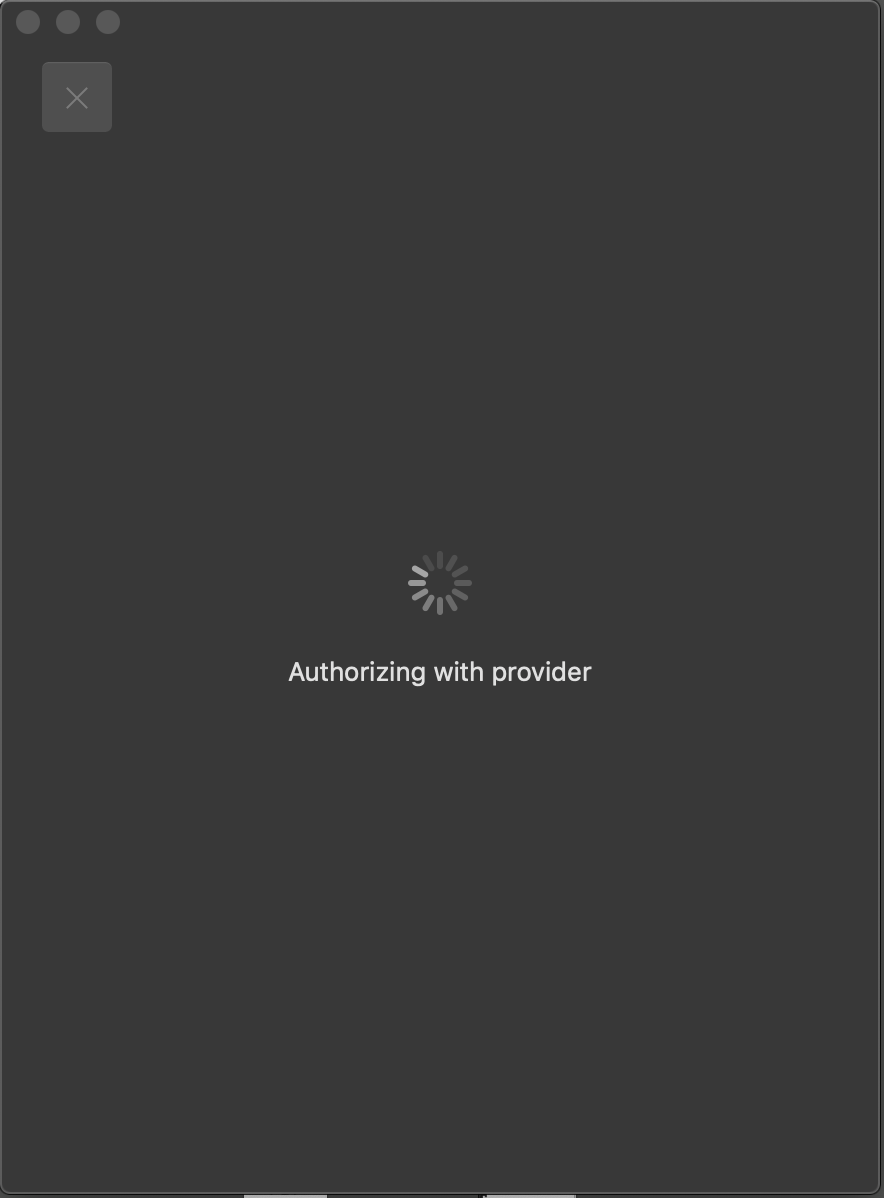
\includegraphics[scale=0.8]{Chapters/images/image7.png}
	
	%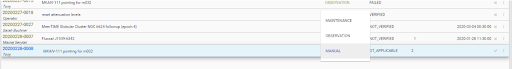
\includegraphics[resolution=100]{bur1.png}
	\caption{MacOS EduVPN connection in progress }
	\label{fig:image7}
\end{figure}
This window will pop-up and press "Approve application"


\begin{figure}[!thb]
	\centering
	%\includegraphicsdpi{100}{}{bur1.png}     
	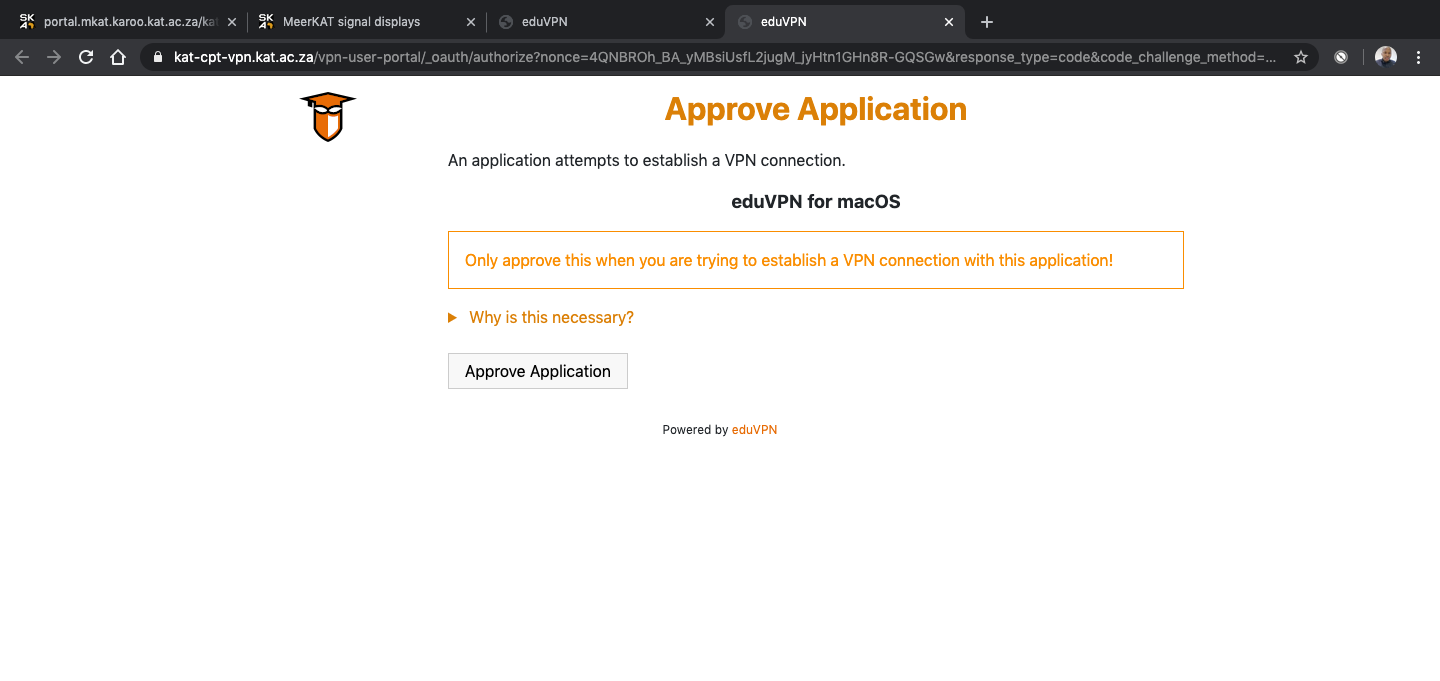
\includegraphics[scale=0.8]{Chapters/images/image26.png}
	
	%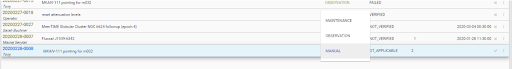
\includegraphics[resolution=100]{bur1.png}
	\caption{MacOS EduVPN aprrove application dialog }
	\label{fig:image26}
\end{figure}










Click connect after approving and the you will be connected

Procedure for Windows
The procedure for connecting to VPN on Windows is more or less the same as that for macOS. 

Download the EduVPN Software for Windows from https://kat-cpt-vpn.kat.ac.za/vpn-user-portal/home
\begin{figure}[!thb]
	\centering
	%\includegraphicsdpi{100}{}{bur1.png}     
	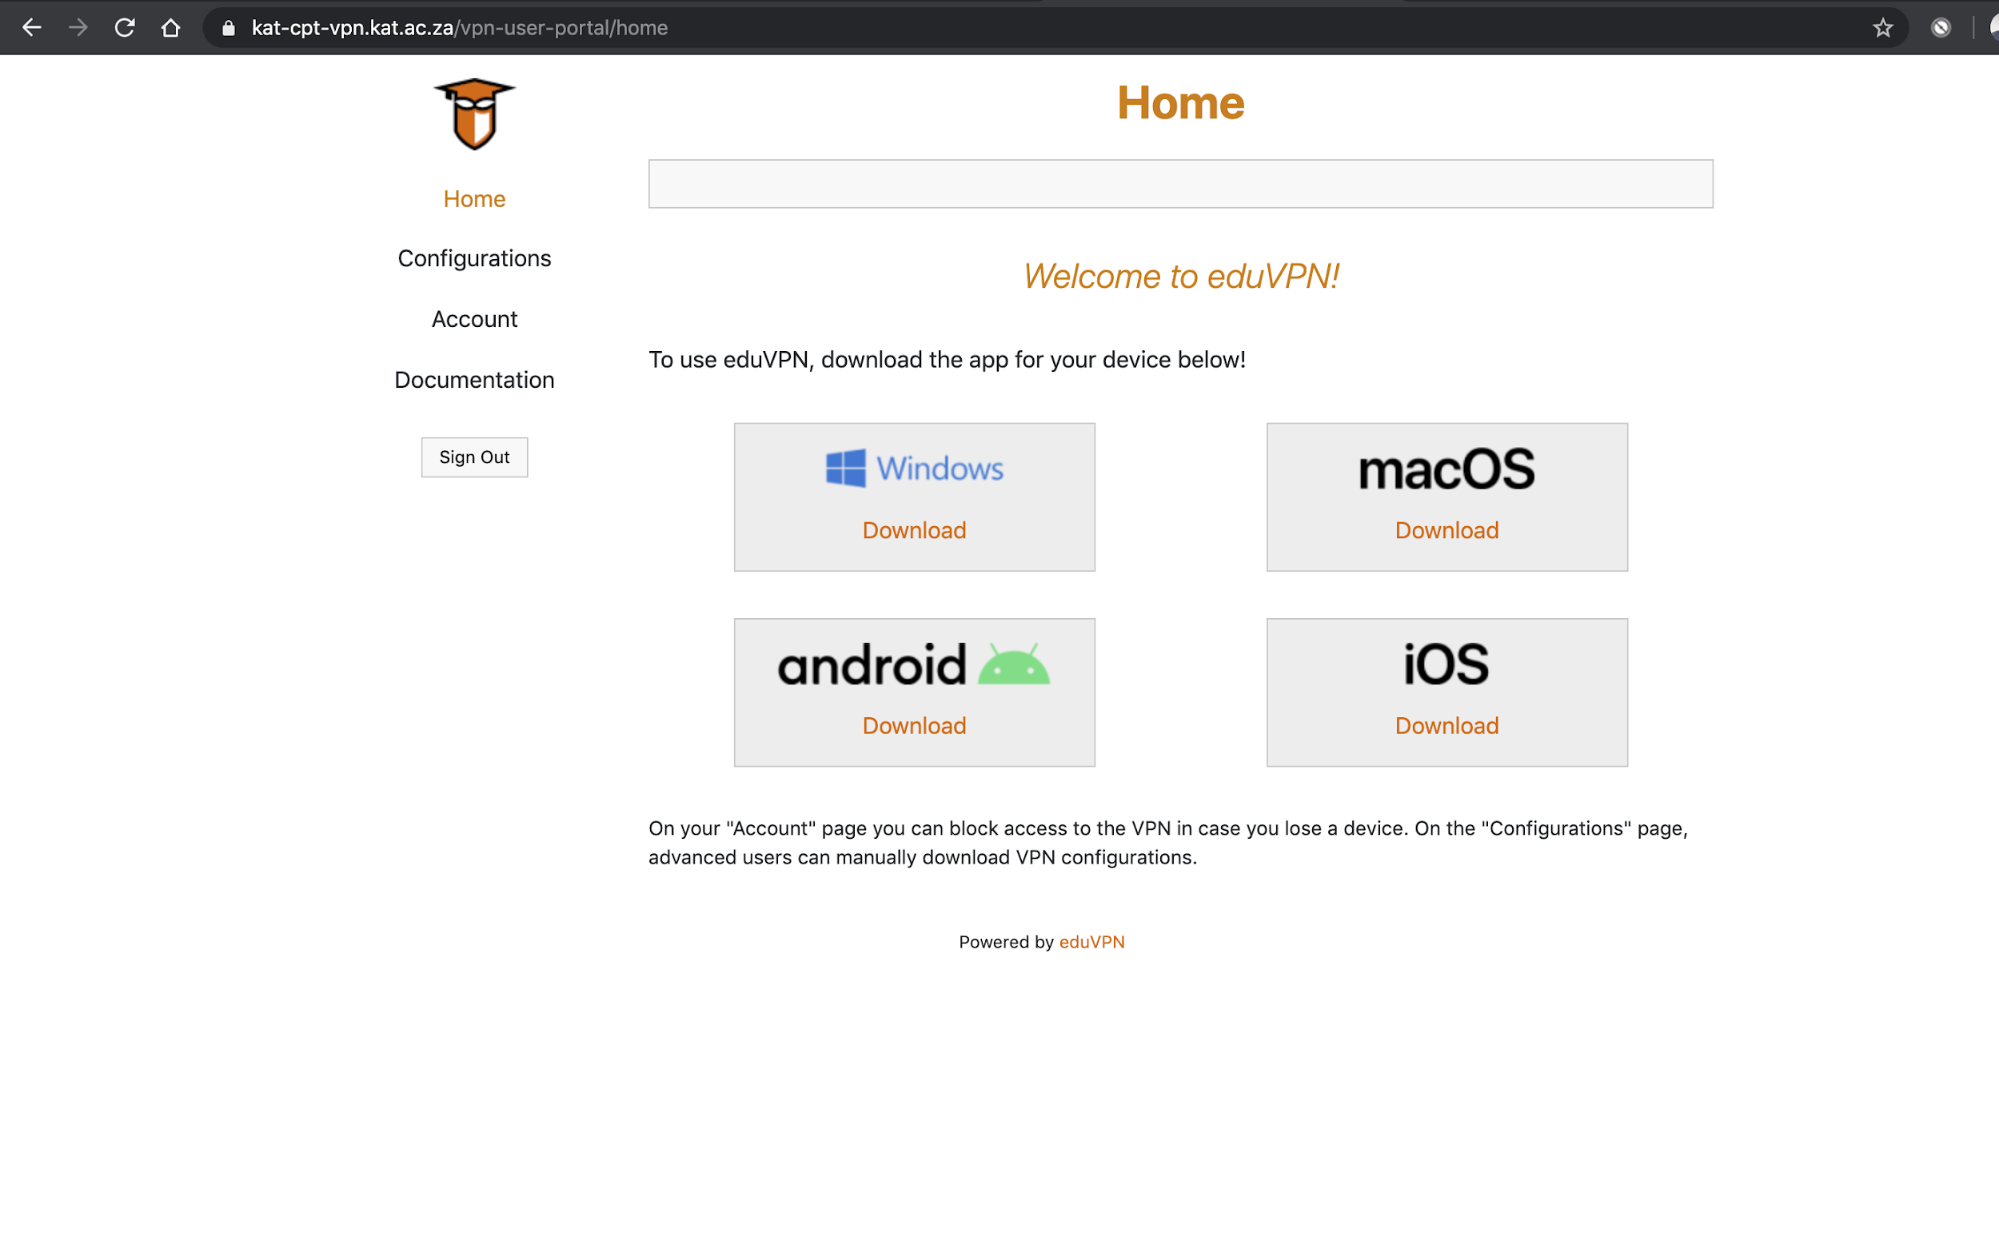
\includegraphics[scale=0.23]{Chapters/images/image106.png}
	
	%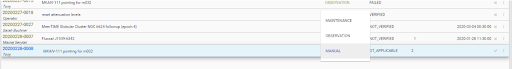
\includegraphics[resolution=100]{bur1.png}
	\caption{CAM GUI approved SB }
	\label{fig:image106}
\end{figure}















The link to the application will be in your downloads folder, click to install.
\begin{figure}[!thb]
	\centering
	%\includegraphicsdpi{100}{}{bur1.png}     
	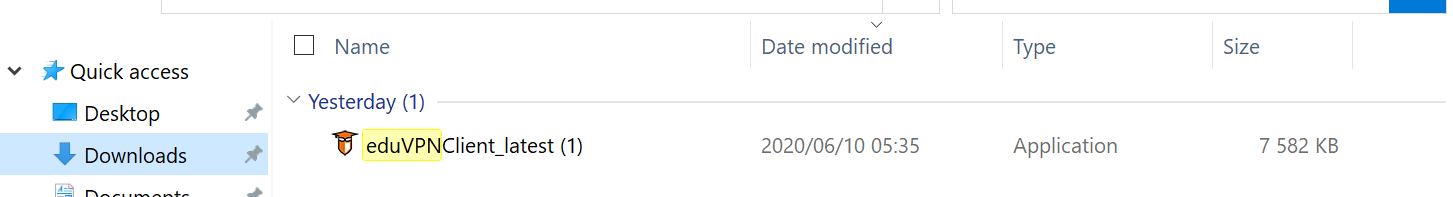
\includegraphics[scale=0.23]{Chapters/images/image8.png}
	
	%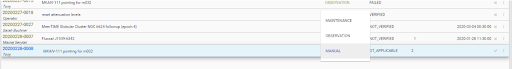
\includegraphics[resolution=100]{bur1.png}
	\caption{MacOS EduVPN connection in progress }
	\label{fig:image8}
\end{figure}
Once the installation is done, you can close the installer and click on the EduVPN item in your start menu to launch VPN
\begin{figure}[!thb]
	\centering
	%\includegraphicsdpi{100}{}{bur1.png}     
	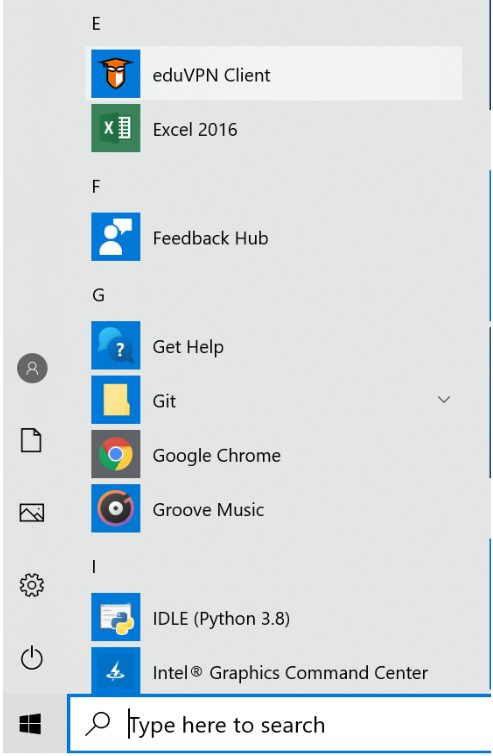
\includegraphics[scale=0.8]{Chapters/images/image28.png}
	
	%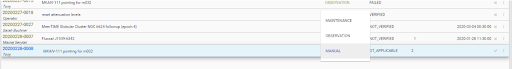
\includegraphics[resolution=100]{bur1.png}
	\caption{MacOS EduVPN connection in progress }
	\label{fig:image28}
\end{figure}

You will be asked how you would like to use VPN, choose ‘Add other address’.
\begin{figure}[!thb]
	\centering
	%\includegraphicsdpi{100}{}{bur1.png}     
	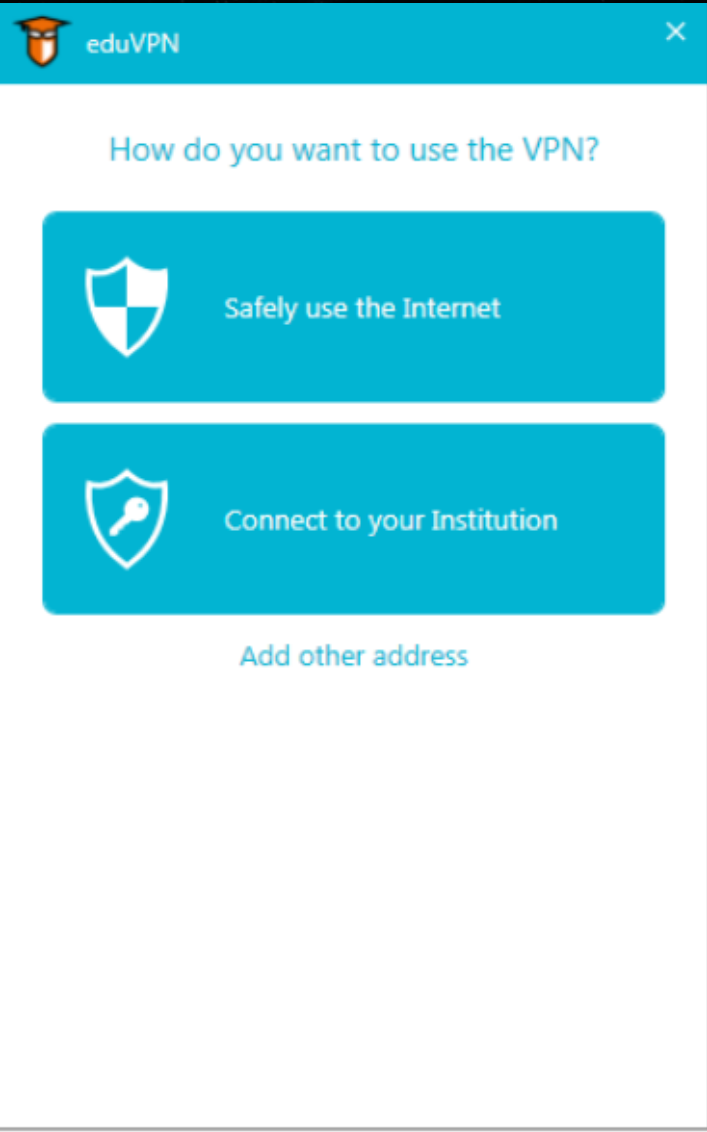
\includegraphics[scale=0.8]{Chapters/images/image110.png}
	
	%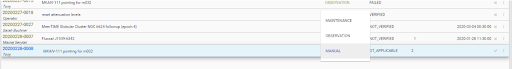
\includegraphics[resolution=100]{bur1.png}
	\caption{MacOS EduVPN connection in progress }
	\label{fig:image110}
\end{figure}
 kat-cpt-vpn.kat.ac.za/ is the URL of our provider, click ‘connect!’ once you are done. 
\begin{figure}[!thb]
	\centering
	%\includegraphicsdpi{100}{}{bur1.png}     
	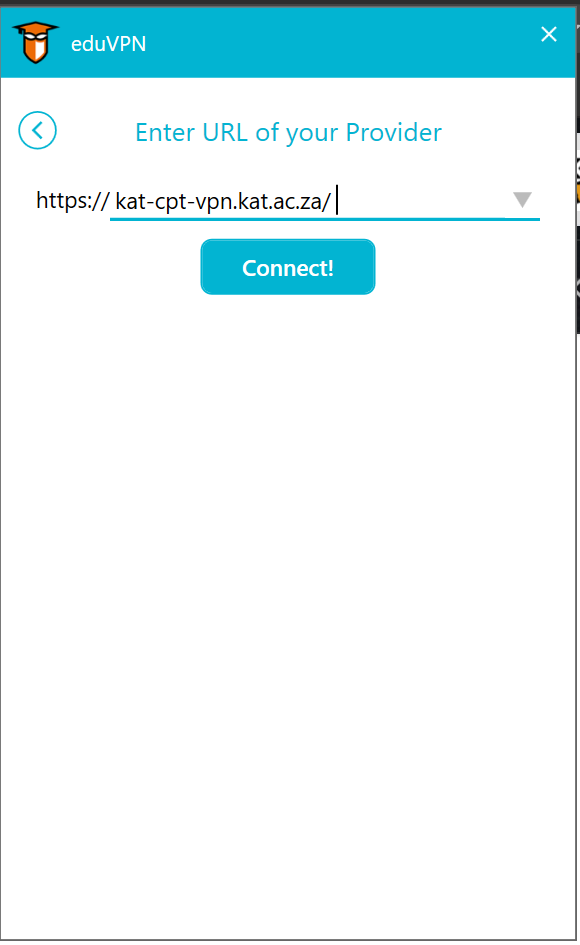
\includegraphics[scale=0.3]{Chapters/images/image69.png}
	
	%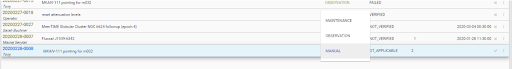
\includegraphics[resolution=100]{bur1.png}
	\caption{MacOS EduVPN connection in progress }
	\label{fig:image69}
\end{figure}
Click ‘SARAO Staff access’
\begin{figure}[!thb]
	\centering
	%\includegraphicsdpi{100}{}{bur1.png}     
	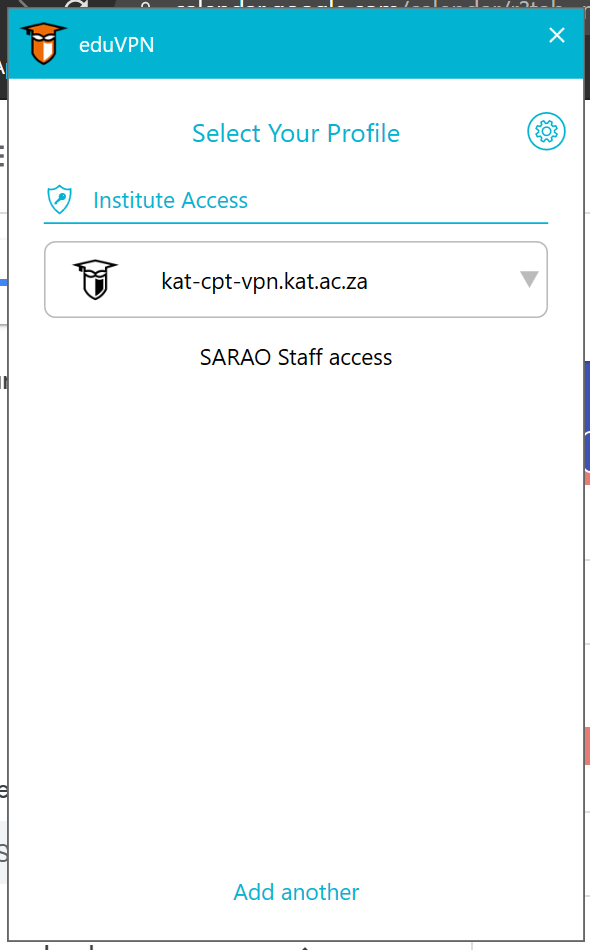
\includegraphics[scale=0.3]{Chapters/images/image111.png}
	
	%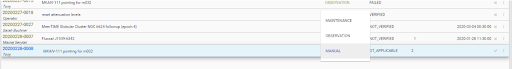
\includegraphics[resolution=100]{bur1.png}
	\caption{MacOS EduVPN connection in progress }
	\label{fig:image111}
\end{figure}
You will be directed to the EduVPN site where you will be required to approve the application like the way you would for macOS. After clicking ‘Approve Application’, you should be connected to VPN
\begin{figure}[!thb]
	\centering
	%\includegraphicsdpi{100}{}{bur1.png}     
	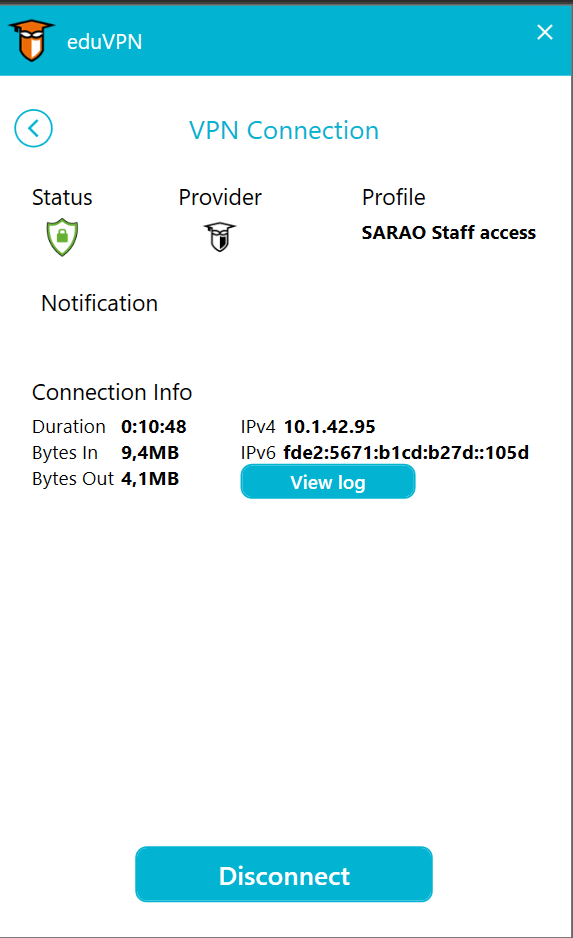
\includegraphics[scale=0.3]{Chapters/images/image58.png}
	
	%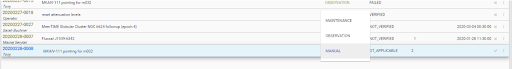
\includegraphics[resolution=100]{bur1.png}
	\caption{MacOS EduVPN connection in progress }
	\label{fig:image58}
\end{figure}

Everytime you want to connect to EduVPN, just click on the item in the start menu as shown in step 3, there will be no need to  enter the URL of the provider. It should automatically appear, all you have to do is repeat step 6.
Don’t forget to remove the old application every time you install a new one by clicking ‘Revoke’ on the EduVPN site. 
\begin{figure}[!thb]
	\centering
	%\includegraphicsdpi{100}{}{bur1.png}     
	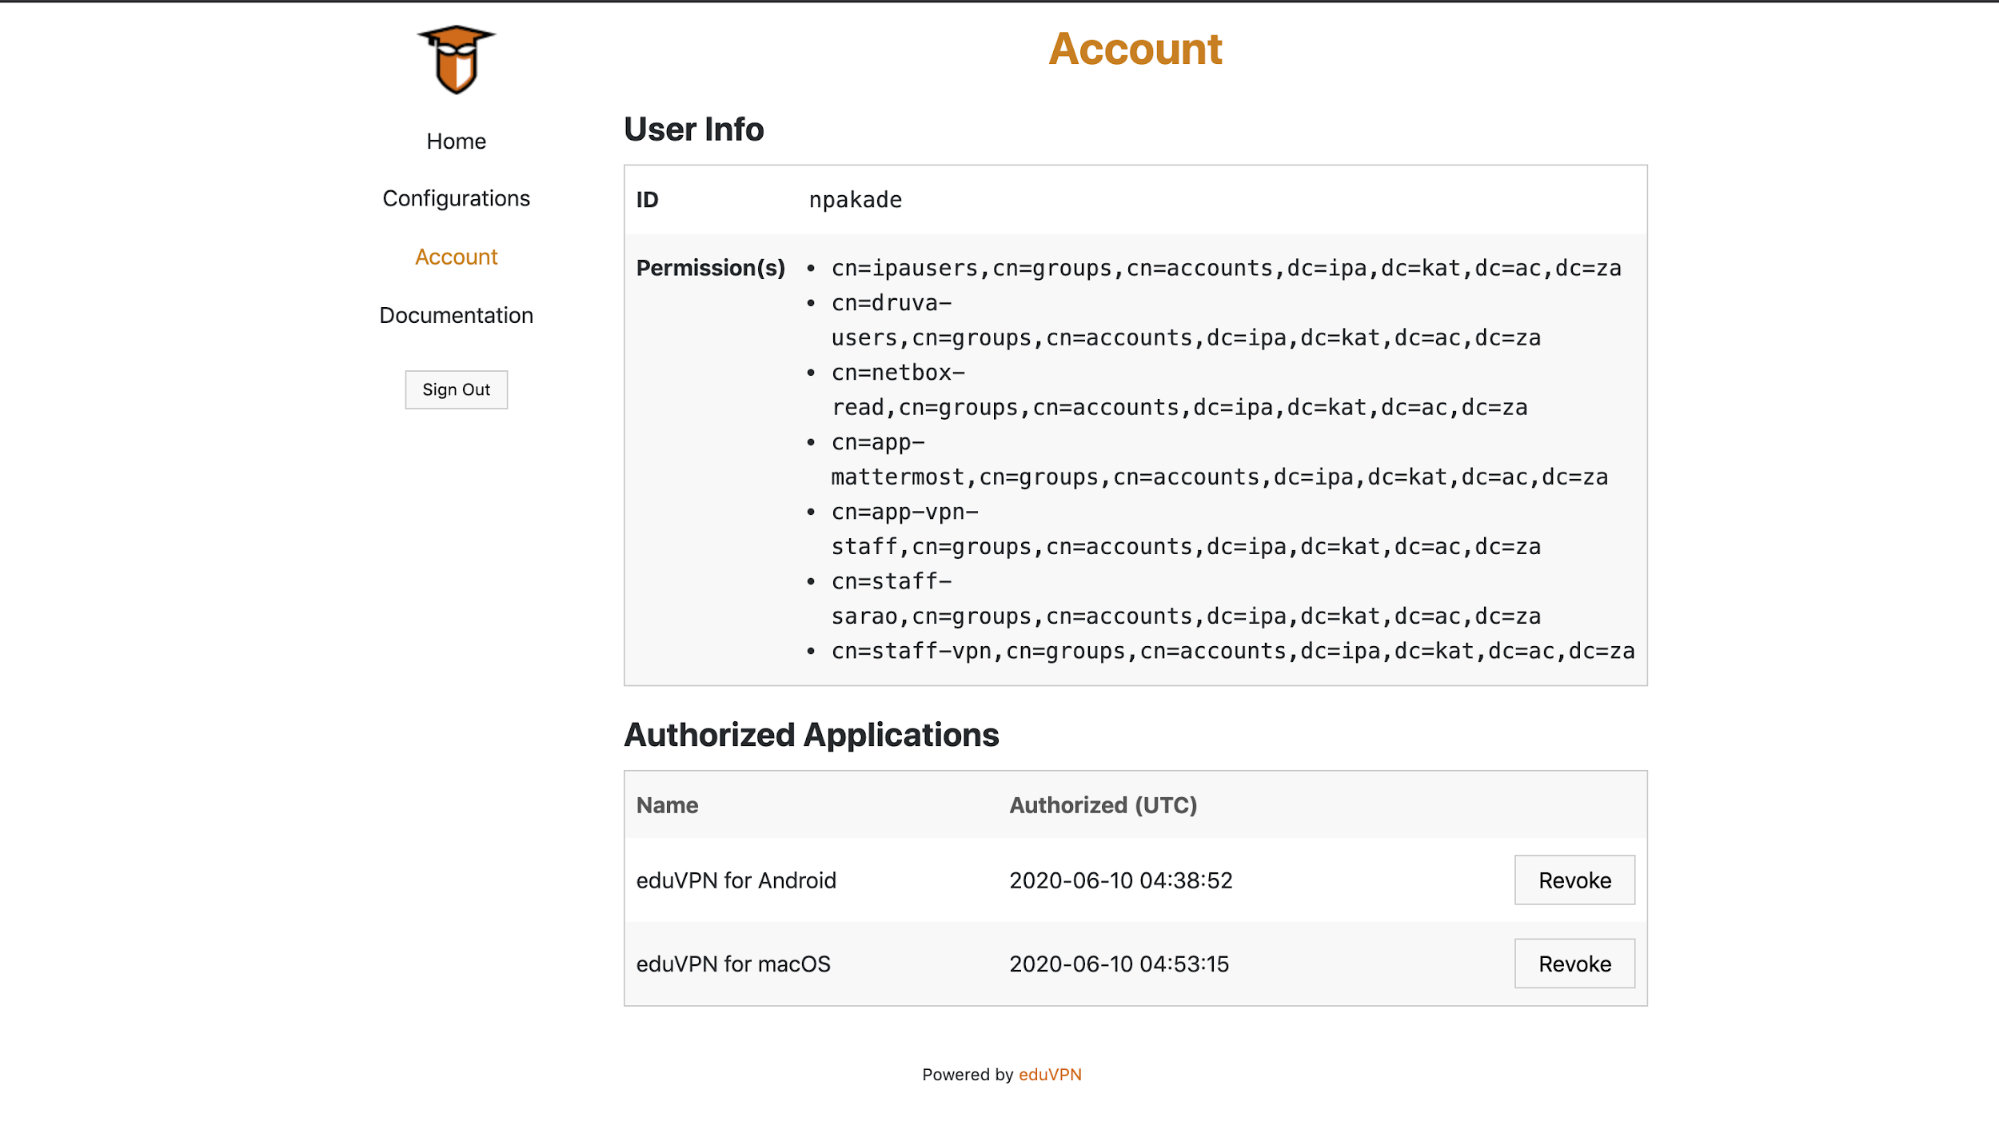
\includegraphics[scale=0.3]{Chapters/images/image32.png}
	
	%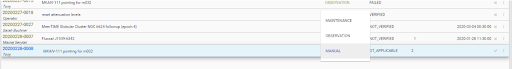
\includegraphics[resolution=100]{bur1.png}
	\caption{MacOS EduVPN connection in progress }
	\label{fig:image32}
\end{figure}
